% !TEX encoding = UTF-8 Unicode
%!TEX root = thesis.tex
% !TEX spellcheck = en-US
%%=========================================
\section{Experiment 2}
In this experiment, the aim is to find a good value for add link probability et al TODO

\subsection{Configuration}



\begin{center}
\begin{longtable}{p{5cm} p{7cm}}
\caption[Experiment configuration]{Experiment configuration} \label{tab:exp1_configuration} \\

\hline \multicolumn{1}{l}{\textbf{Parameter}} & \multicolumn{1}{l}{\textbf{Value}} \\ \hline 
\endfirsthead

\multicolumn{2}{c}%
{{\bfseries \tablename\ \thetable{} -- continued from previous page}} \\
\hline \multicolumn{1}{l}{\textbf{Parameter}} & \multicolumn{1}{l}{\textbf{Value}} \\ \hline 
\endhead

\hline \multicolumn{2}{r}{{Continued on next page}} \\ \hline
\endfoot

\hline \hline
\endlastfoot

Number of generations & 50 \\
\midrule
Fitness function & Local similarity, as described in experiment 1 \\
\midrule
Target sound & Drum loop \\
\midrule
Input sound & White noise \\
\midrule
Effect & Distortion and resonant low-pass filter \\
\midrule
Audio features & mfcc\_0, mfcc\_0\_\_derivative, mfcc\_1 \\
\midrule
Number of runs & 400 per configuration \\
\end{longtable}
\end{center}

\subsection{Evaluation of configurations}
Figure \ref{fig:add_link_probability} TODO shows that 0.03 is probably the best value while 0.3 is significantly worse

\begin{figure}[h]
    \centering
    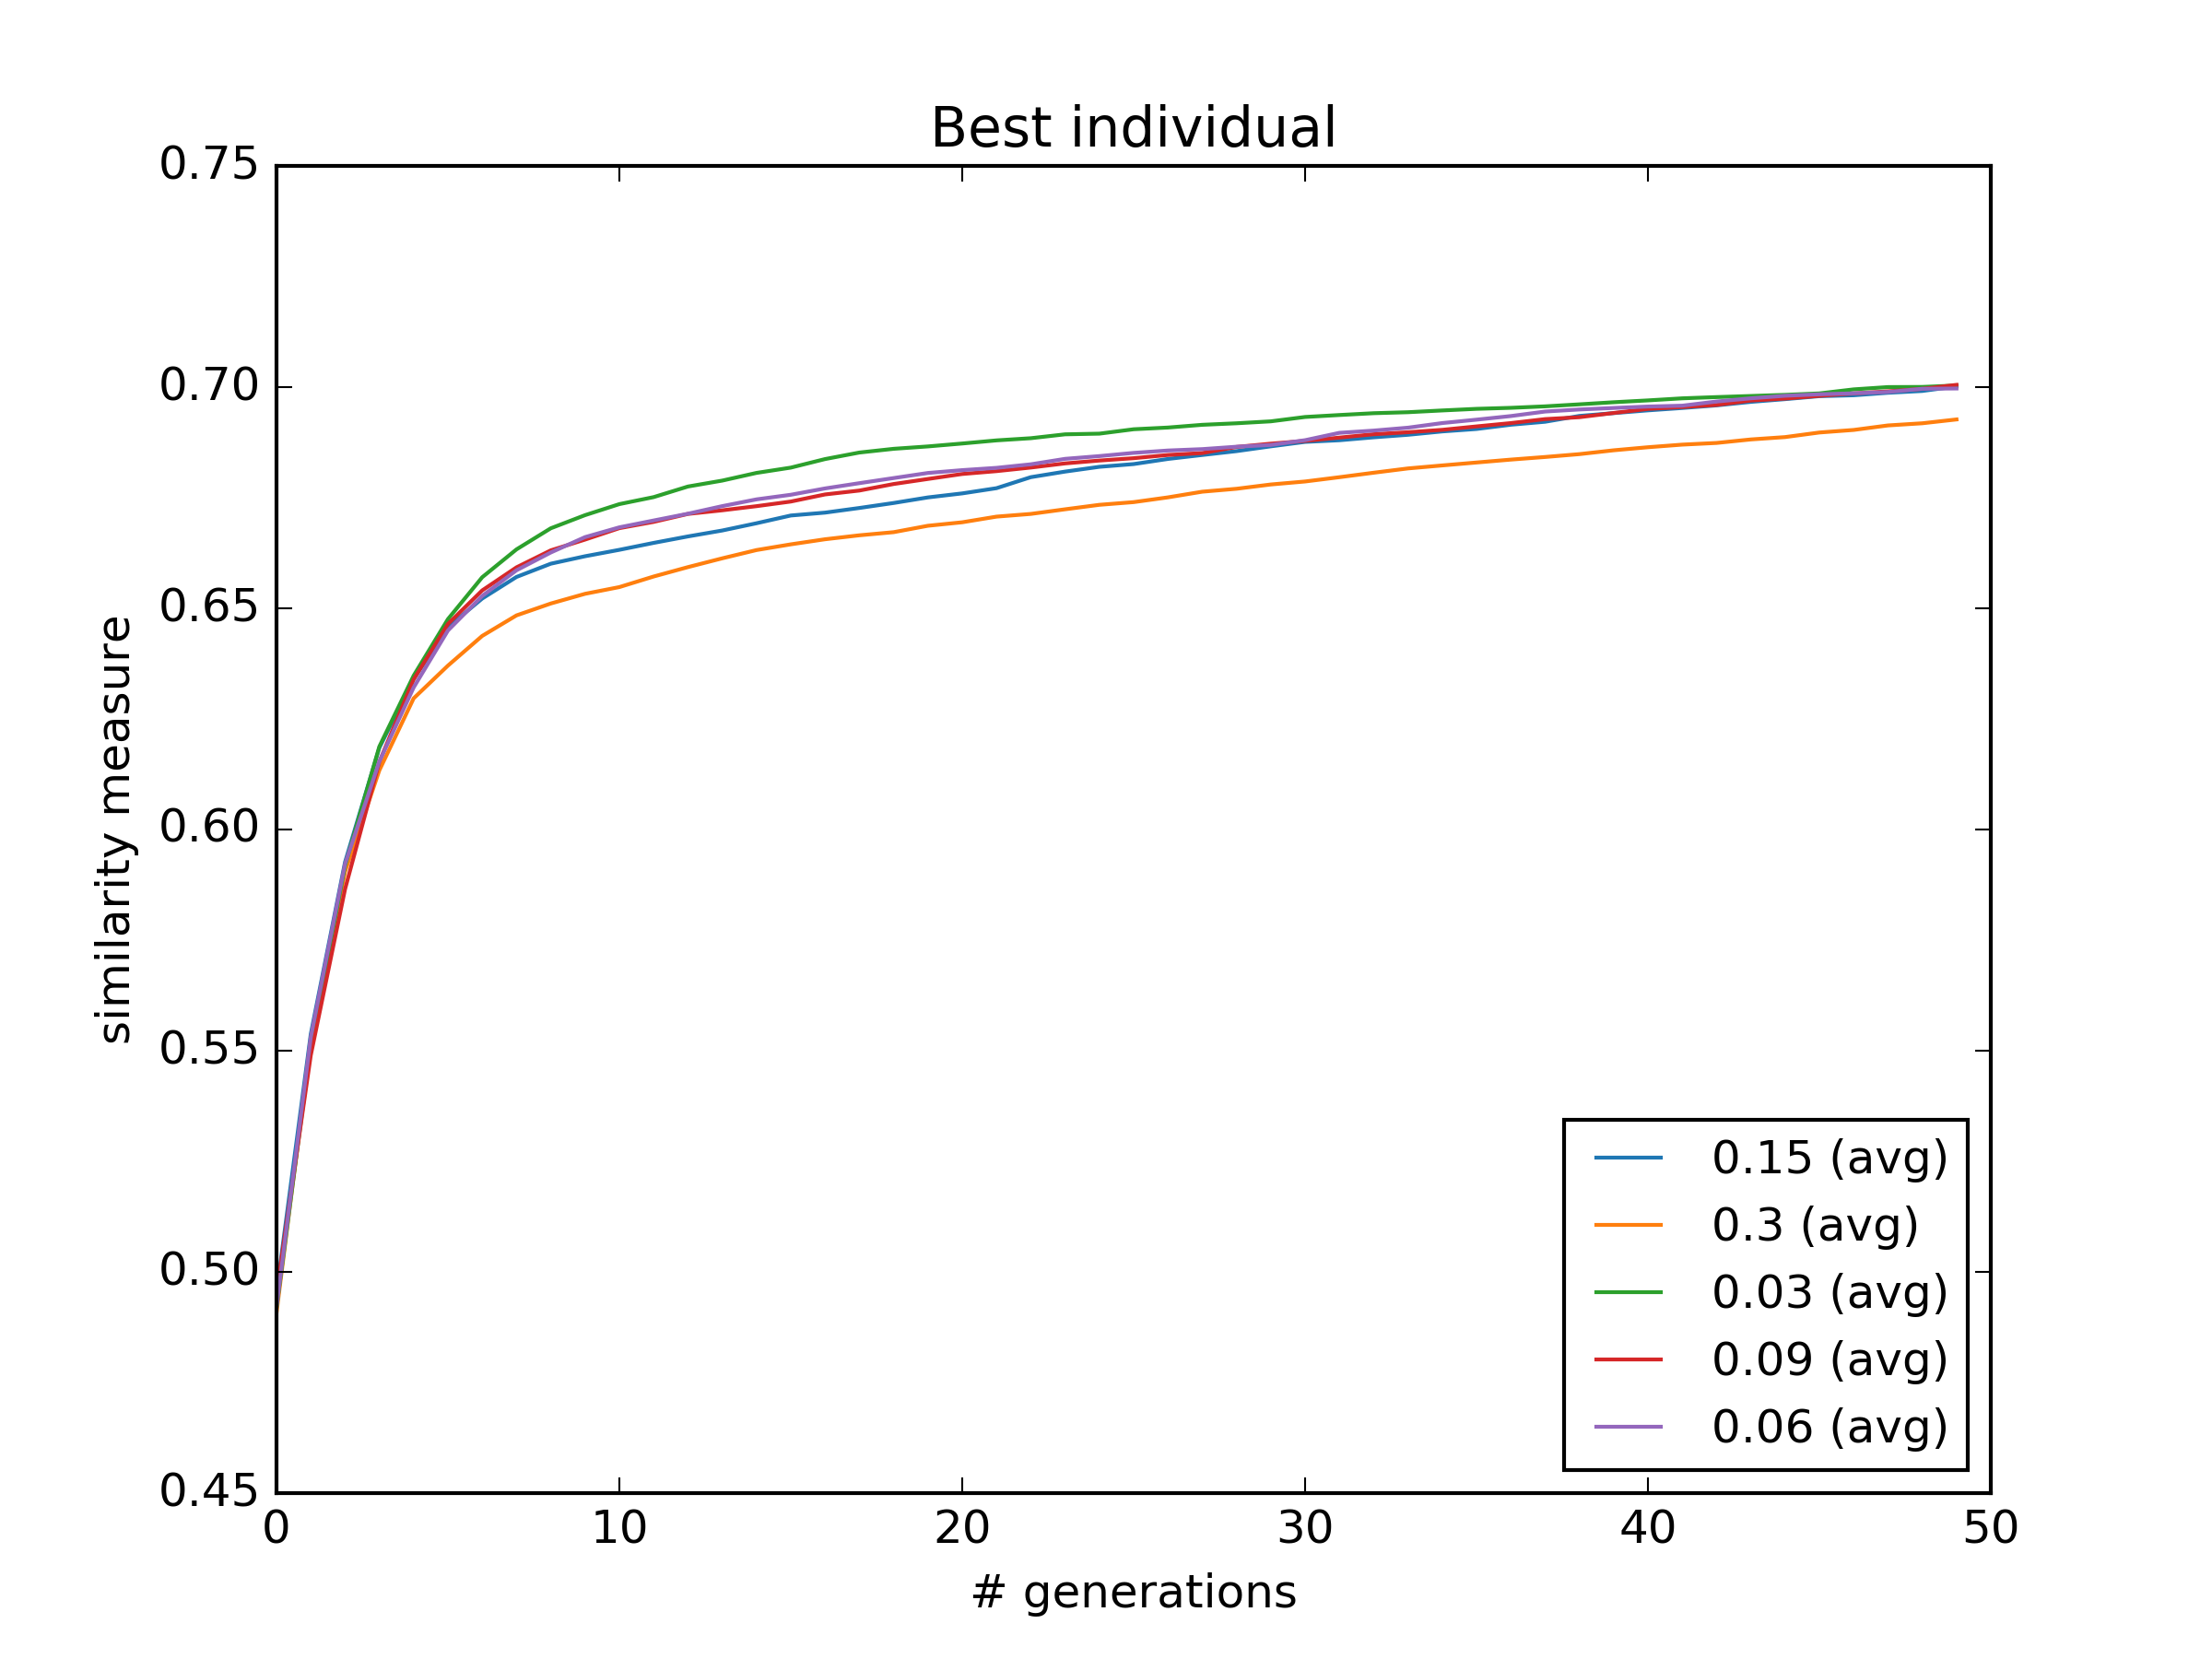
\includegraphics[width=0.99\textwidth]{add_link_probability}
    \caption{TODO caption}
    \label{fig:add_link_probability}
\end{figure}

TODO: Show typical end-result neural networks from all the configurations, to highlight that higher probability builds a larger, more complex network